\section{实验与结果分析}

\subsection{实验设置与对比方法}

本文所有实验均在基于Ubuntu 20.04操作系统的Kaggle Notebook环境完成,硬件配置采用Kaggle提供的单张NVIDIA P100 GPU(16GB显存)和30GB RAM内存。实验模型代码基于PyTorch框架搭建,同时搭配CUDA 11.3加速库加速模型训练。

模型的网络权重的初始化采用He normal,并使用初始学习率为$1 \times 10^{-4}$的Adam优化器更新权重。每个实验的训练轮数设置为100个Epoch(本章中简称Ep),且在每轮训练结束后在验证集上进行模型评估,保存Dice得分最高的模型权重。

本文在进行模型评估时,以Dice系数作为核心评价指标,用于衡量模模型在分割任务中预测结果与真实标签之间的重叠程度,是医学图像分割中最常用且最敏感的评估指标之一。为了更全面地反映模型性能,辅以Jaccard指数、F1分数、Accuracy、Precision与Recall等多维度指标进行综合评估。

\subsection{消融和增广实验}

本研究开展一系列消融实验,围绕模型结构、损失函数以及训练策略三个层面进行,来系统评估各改进模块对模型语义分割性能所产生的影响,实验以基准U-Net模型(后文简称基准模型)作为对照组,之后逐步引入或者移除关键组件,这些关键组件覆盖跳跃连接、注意力机制、数据提高策略以及不同的损失函数组合,以此来观察每项设计对模型性能的独立贡献以及协同增益情况,为构建最终的优化模型AAH U-Net提供理论依据和实验数据支持。

所有消融与增广实验均使用ISIC 2018,按照8:2的比例划分训练集与验证集,并且在固定的模型训练框架以及超参数设置下进行公平比较。

\subsubsection{基准模型性能验证}

在所有实验中,基准模型使用原始U-Net网络结构,配合混合损失函数和Adam优化器进行训练,关于损失函数和优化器的具体参数设置已在第三章阐述。此外,基准模型的训练未采用任何形式的数据增强或正则化操作,以便纯粹评估其建模能力与收敛特性。

为全面评估基准 U-Net 模型在验证集上的性能表现,图~\ref{fig:base_unet_metrics} 展示了训练过程中多个关键评估指标(包括 Dice 系数、Jaccard 指数、Accuracy、Precision、Recall、F1-Score、Specificity 及 Loss)随 epoch 变化的趋势曲线。训练曲线反映了模型收敛过程及其在训练与验证集上的性能差异,可用于分析模型的拟合能力与泛化效果。

\begin{figure}[!htbp]
    \centering
    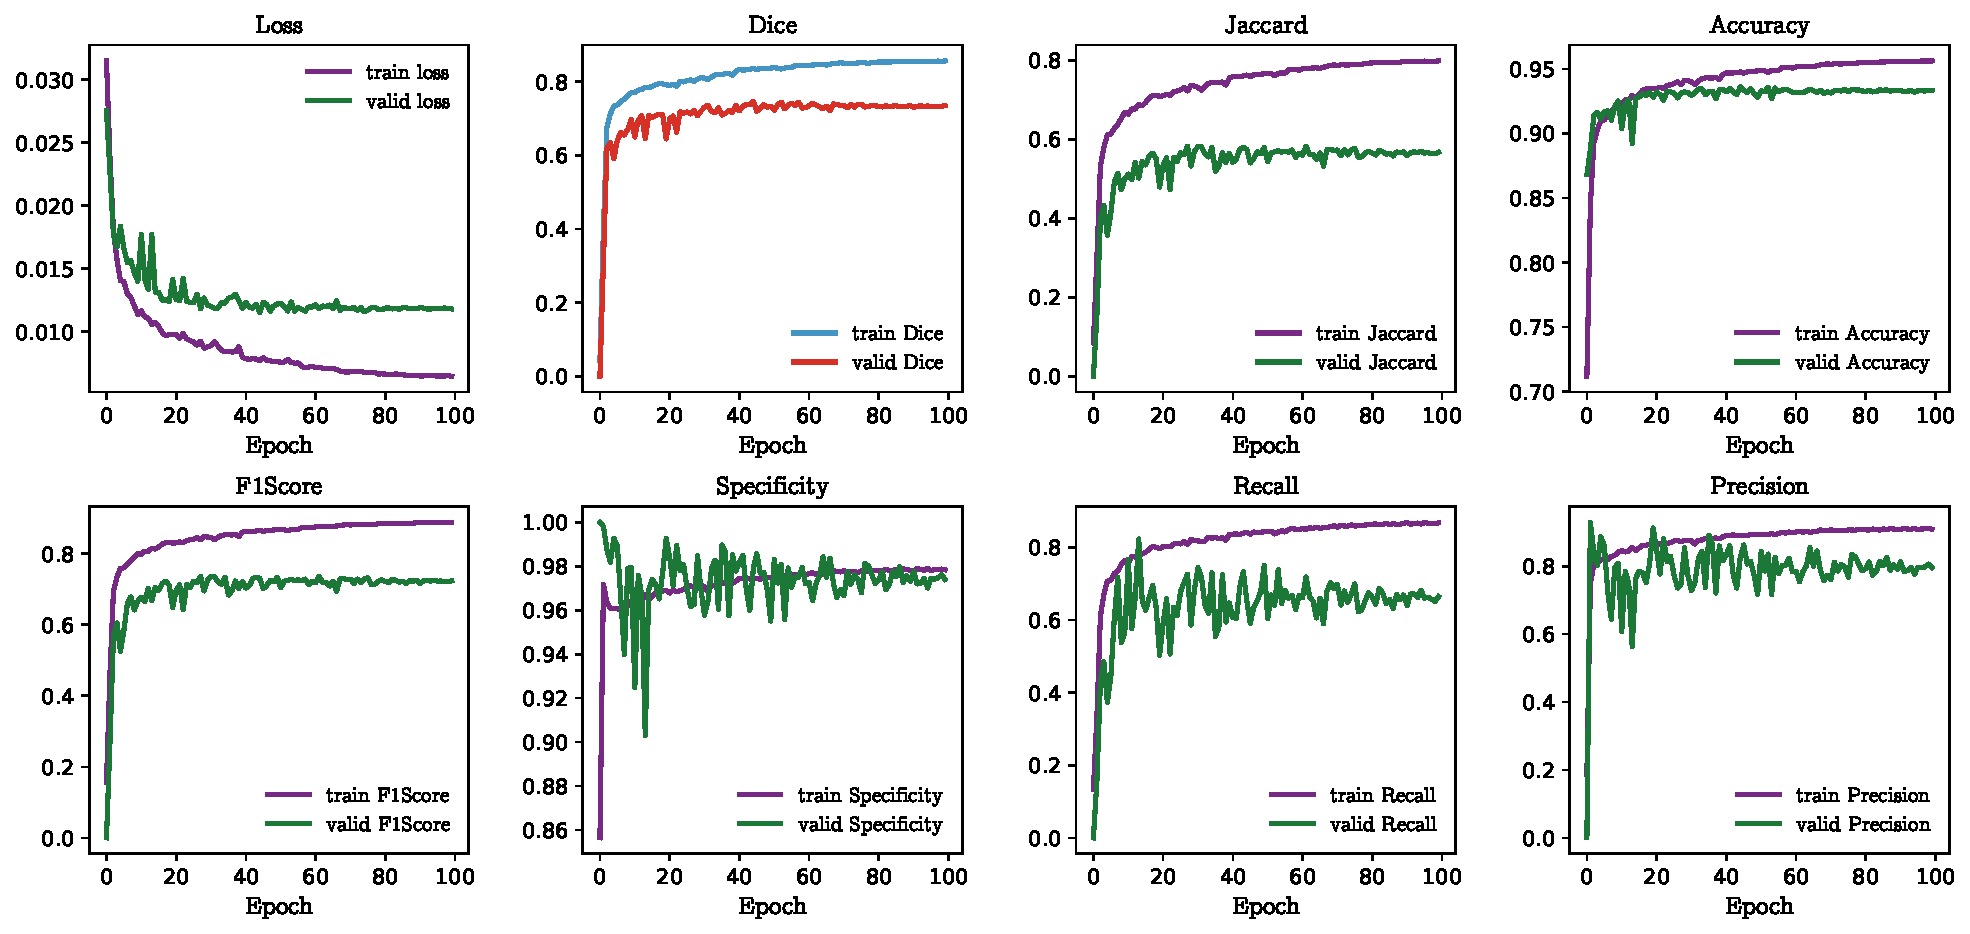
\includegraphics[width=\textwidth]{fig/base_unet_metrics.pdf}
    \caption{基准模型训练过程中的性能指标变化趋势}
    \label{fig:base_unet_metrics}
\end{figure}

表 \ref{tab:unet_epoch_compare} 对比了基准模型在验证集上的三个关键时间点——首次达到 Dice ≥ 0.70 的第 13 轮、全局最优的第 45 轮以及训练末期(最后 10 轮)——对应的主要性能指标。可以看到,模型在第 13 个 epoch 即取得 0.7077 的 Dice值 和 0.5420 的 Jaccard值,说明其收敛速度较快。随后经过 32 轮的渐进优化,Dice 进一步提升到 0.7469(+3.9 pp),Jaccard 则提升到 0.5747(+3.3 pp),而 Precision 几乎保持不变(≈ 0.826),表明网络 在保证低假阳性的同时显著减少漏检。Val-Loss 同期下降约 12 \%,与性能上升趋势一致。

此外,末 10 轮的均值与标准差(右侧一列)显示各指标波动极小(Dice σ ≈ 0.001),证明模型已进入稳定收敛区间且未出现明显过拟合。基于这一观察,本文后续将第 45 轮作为“最优性能”参考点,而第 13 轮则可作为“早期收敛效率”的对照基准,用以衡量不同改进策略在早期与最终阶段的综合效益。

\begin{table}[htbp]
    \centering
    \caption{基准模型关键Epoch验证集性能指标对比}
    \label{tab:unet_epoch_compare}
    \begin{tabular}{lcccc}
        \toprule
        指标 (val) & Epoch 13 & Epoch 45 (best) & $\Delta$ & 末10轮均值与标准差 \\
        \midrule
        Dice        & 0.7077 & \textbf{0.7469} & +3.9 pp   & 0.734 $\pm$ 0.001 \\
        Jaccard     & 0.5420 & \textbf{0.5747} & +3.3 pp   & 0.561 $\pm$ 0.002 \\
        Precision   & \textbf{0.8266} & 0.8262 & $\approx$0 & 0.822 $\pm$ 0.008 \\
        Recall      & 0.6266 & \textbf{0.6537} & +2.7 pp   & 0.645 $\pm$ 0.010 \\
        Val-Loss $\downarrow$ & 0.01312 & \textbf{0.01150} & 0.00162 & 0.0117 $\pm$ 0.0002 \\
        \bottomrule
    \end{tabular}
\end{table}

\subsubsection{跳跃连接的结构消融实验}

为了评估跳跃连接在 U-Net 网络中的作用,参考Drozdzal等人\cite{drozdzal2016}对于U-Net网络中跳跃连接重要性的研究,本文设计了删除跳跃连接后的U-Net模型(简称Skipless模型)的消融实验,并得到了删除跳跃连接后的模型训练指标趋势图~\ref{fig:skipless_unet}。

\begin{figure}
    \centering
    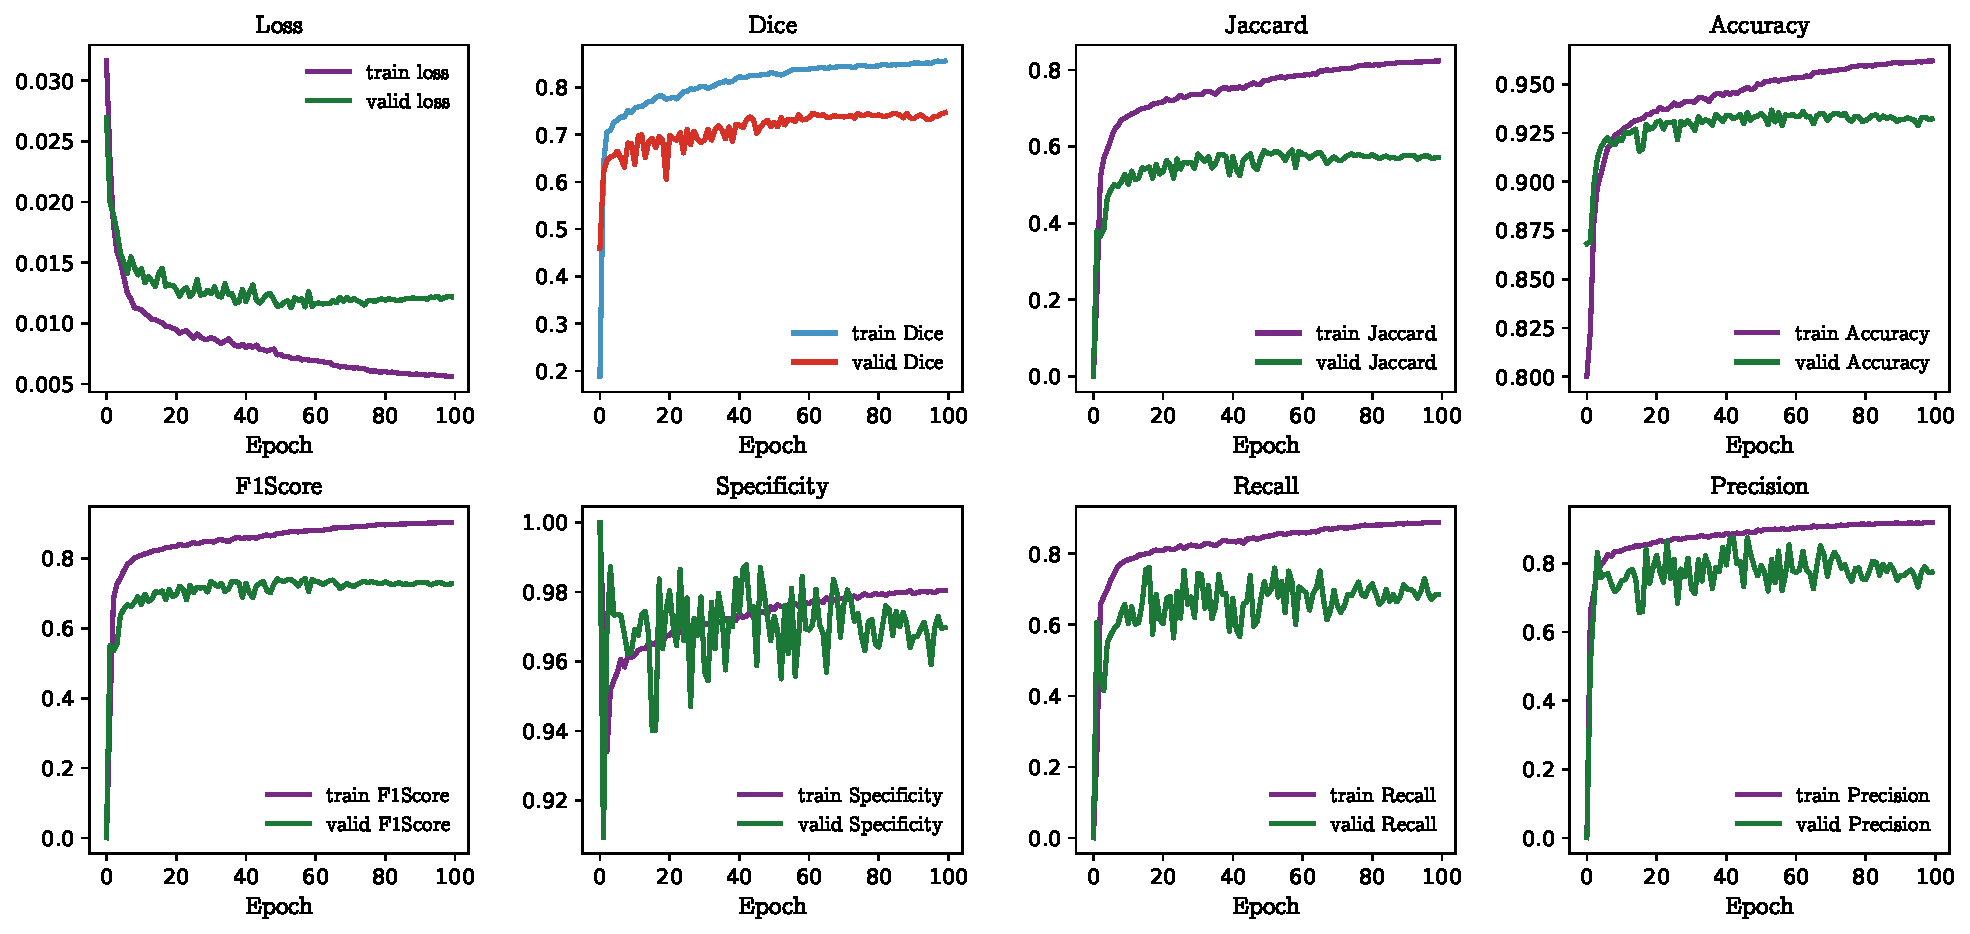
\includegraphics[width=0.9\textwidth]{fig/skipless_unet_metrics.pdf}
    \caption{删去跳跃连接后的U-Net模型训练指标趋势}
    \label{fig:skipless_unet}
\end{figure}

表~\ref{tab:ablation_skip_connection}展示了基准模型和Skipless模型在最优验证Dice的epoch时,各评价指标的值。从数据上看,Skipless模型在 Dice、F1-score 与 Jaccard 等综合性能指标上实现了小幅提升,分别提高了 1.4\%、2.8\% 与 4.6\%。与此同时,验证损失同步下降,说明模型在删去跳跃连接后未造成训练过程的不稳定或过拟合恶化。

\begin{table}[htbp]
    \centering
    \caption{基准模型与Skipless模型在验证集上的性能对比}
    \label{tab:ablation_skip_connection}
    \begin{tabular}{lcccc}
        \toprule
        指标(Val) & 基准模型(Ep45) & Skipless模型 & $\Delta$ & 相对变化 \\
        \midrule
        Dice         & 0.7469 & \textbf{0.7576} & +0.0107 & +1.4\% \\
        F1           & 0.7299 & \textbf{0.7507} & +0.0208 & +2.8\% \\
        IoU / Jaccard & 0.5747 & \text{0.6009} & +0.0262 & +4.6\% \\
        Precision    & \textbf{0.8262} & 0.8009 & $-$0.0253 & $-$3.1\% \\
        Recall       & 0.6537 & \textbf{0.7064} & +0.0527 & +8.1\% \\
        Accuracy     & \textbf{0.9362} & 0.9352 & $-$0.0010 & $-$0.1\% \\
        Specificity  & \textbf{0.9791} & 0.9719 & $-$0.0072 & $-$0.7\% \\
        Val-Loss $\downarrow$ & 0.01150 & \textbf{0.01114} & $-$0.00036 & $-$3.1\% \\
        \bottomrule
    \end{tabular}
\end{table}


进一步分析发现,Skipless模型在 Recall 指标上显著提升了8.1\%,而 Precision 与 Specificity 分别下降了 3.1\% 与 0.7\%。这一现象表明在未使用跳跃连接的情况下,模型更倾向于扩大预测区域,更“激进”地标注前景区域,在减少漏检的同时带来了更多误检。

结合前面章节中对U-Net中的跳跃连接结构机制分析可知,跳跃连接将浅层网络中的高分辨率纹理特征直接拼接至解码器端,增强了分割边界的保留与精度。而在跳跃连接被删除后,模型必须依赖上采样的深层语义特征来重建图像细节,结果导致预测边界变得更加平滑甚至过度扩张。这一结论与 FCN 系列研究中对跳跃连接的功能归因一致,即跳跃连接能显著提升边界分割精度与早期特征利用效率\cite{milletari2016}。

综上,针对ISIC2018 皮肤病变的语义分割任务,跳跃连接并非模型性能的必要条件。在某些关注 Recall 的场景下,去除跳跃连接反而可带来一定的性能提升。然而,在对误诊率要求较高的临床应用中,保留跳跃连接仍是更稳妥的选择。

\subsubsection{损失函数的混合消融实验}

为了验证不同损失函数策略对模型性能的影响,本文共对三种损失函数方案进行了系统性的消融对比:基准模型使用DiceLoss和CrossEntropyLoss等权加权的混合损失(HybridLoss),另设两组对照实验分别采用 DiceLoss 与 CrossEntropyLoss。在本节中,对照实验方案简称为C组(CrossEntropyLoss)和D组(DiceLoss)。

\begin{table}[htbp]
    \centering
    \caption{不同损失函数下模型性能对比}
    \label{tab:loss_ablation}
    \begin{tabular}{lcccccc}
        \toprule
        指标(Val) & 基准模型(Ep45) & D (Ep 99) & C (Ep 78) & $\Delta$ D$-$B & $\Delta$ C$-$B \\
        \midrule
        Dice        & 0.747 & 0.747 & \textbf{0.752} & $-$0.0004 & +0.0046 (+0.6\%) \\
        F1-score    & 0.730 & 0.734 & \textbf{0.740} & +0.004 & +0.010 \\
        Jaccard     & 0.575 & 0.580 & \textbf{0.588} & +0.005 & +0.013 \\
        Precision   & \textbf{0.826} & 0.801 & 0.776 & $-$0.025 & $-$0.050 \\
        Recall      & 0.654 & 0.677 & \textbf{0.708} & +0.024 & +0.054 \\
        Accuracy    & \textbf{0.936} & 0.935 & 0.934 & $-$0.001 & $-$0.002 \\
        Specificity & \textbf{0.979} & 0.975 & 0.969 & $-$0.004 & $-$0.010 \\
        \bottomrule
    \end{tabular}
\end{table}


在验证集最佳 Dice值所在 Epoch 下,三种方案的表现如表~\ref{tab:loss_ablation} 所示。从数据中可以分析出来,C组在顶峰Dice值上略超B组,但Recall值大幅提升,表明通过CrossEntropyLoss对每个像素均衡优化,鼓励网络捕获更多前景,使得捡漏更少,但是因为正负样本的不平衡使得Precision下滑。而由于DiceLoss梯度在早期预测极偏时接近0,使得D组的模型收敛明显变慢。

综上,混合损失函数是综合最稳健的折中,峰性能仅次于D组0.6 \%,却保持 Precision 与 Specificity 最佳。C组适用于追求高召回率的场景,例如早期筛查、提高敏感度。D组综合性能最差,仅采用DiceLoss使得模型训练变慢,晚期训练波动变大。

\subsubsection{数据增强增广实验}

为验证数据增强策略在本研究任务中的有效性,本节将采用了数据增强(水平翻转、垂直翻转和随机旋转)的U-Net模型(简称Augment U-Net)与基准模型在验证集上的全局最优性能进行对比,具体结果如表~\ref{tab:augment_best}所示。

\begin{table}[htbp]
    \centering
    \caption{基准模型 与Augment U-Net在验证集最佳 Epoch 下的性能对比}
    \label{tab:augment_best}
    \begin{tabular}{lcccc}
        \toprule
        指标(Val) & 基准模型(Ep45) & Augment U-Net(Ep 44) & $\Delta$ & 相对提升 \\
        \midrule
        Dice        & 0.7469 & \textbf{0.7624} & +0.0155 & +2.1\% \\
        F1-score    & 0.7299 & \textbf{0.7481} & +0.0182 & +2.5\% \\
        Jaccard     & 0.5747 & \textbf{0.5939} & +0.0192 & +3.3\% \\
        Precision   & \textbf{0.8262} & 0.7429 & $-$0.0833 & $-$10.1\% \\
        Recall      & 0.6537 & \textbf{0.6816} & +0.0279 & +4.3\% \\
        Accuracy    & 0.9362 & \textbf{0.9399} & +0.0037 & +0.4\% \\
        Specificity & \textbf{0.9791} & 0.9772 & $-$0.0019 & $-$0.2\% \\
        Val-Loss $\downarrow$ & 0.01150 & \textbf{0.01011} & $-$0.00139 & $-$12.1\% \\
        \bottomrule
    \end{tabular}
\end{table}

通过对结果进行数据分析,采用数据增强在一定程度上提升了模型的整体性能,多项指标值均小幅提升。进一步分析发现,Augment U-Net模型出现了Precsion-Recall权衡效应:模型的召回率Recall由 0.6537 显著提高至 0.6816,而与此同时精度Precision则从 0.8262 降至 0.7429。

%此外,通过统计训练末尾5个 epoch(Tail-5)的验证 Dice 均值与方差发现:Augment U-Net模型 Tail-5 均值为 0.723,方差为 0.013,而 基准模型 分别为 0.700 和 0.023,表明数据增强改善的是最终表示能力与过拟合抑制。

综上,在本研究中,数据增强作为一种低成本、易实施的性能增益策略,在不增加模型结构复杂度的前提下,即可实现模型性能的稳定提升并且抑制过拟合现象。

\subsubsection{注意力机制增广实验}

在评估跳跃连接引入注意力机制对模型性能的提升效果的增广实验中,引入注意力机制的U-Net模型(简称Attention U-Net)在多个关键指标上取得了显著性能提升。

\begin{table}[htbp]
    \centering
    \caption{基准模型 与 Attention U-Net模型在验证集上的性能对比}
    \label{tab:att_unet}
    \begin{tabular}{lcccc}
        \toprule
        指标(Val) & 基准模型 (Ep45) & Attention U-Net (Ep 38) &  $\Delta$ & 相对提升 \\
        \midrule
        Dice        & 0.747 & \textbf{0.818} & +0.071 & +9.5\% \\
        Jaccard     & 0.575 & \textbf{0.655} & +0.091 & +15.8\% \\
        Precision   & \textbf{0.826} & 0.808 & $-$0.018 & $-$2.3\% \\
        Recall      & 0.654 & \textbf{0.791} & +0.137 & +21.0\% \\
        Accuracy    & \textbf{0.936} & 0.948 & +0.011 & +1.2\% \\
        Loss $\downarrow$ & 0.0115 & \textbf{0.0105} & $-$0.0010 & $-$8.8\% \\
        \bottomrule
    \end{tabular}
\end{table}

如表~\ref{tab:att_unet} 所示,其验证 Dice 提高了 7.1 个百分点,相对提升达 9.5\%,Jaccard 指标同步增长 15.8\%,说明跳跃连接处的注意力模块让解码端自适应加权高/低层特征,改善边界细节与类间分离度。除此之外,Recall 提升幅度尤为显著,达 21.0\%。相较之下,Precision 略微下降(–2.3\%),说明该模型更敢于召回难分割的像素,用少量的Precision损失换来明显捡漏减少,这一策略在临床早期筛查中更安全。

同时图~\ref{fig:attunet}还显示出Attention U-Net的收敛速度显著加快:在首个 epoch 即可达到 Dice ≥ 0.70 的水平,表明注意力机制增强了前向通路的信息聚合效率,并为反向传播提供了更有效的梯度信号。

%而且在训练后期的尾部稳定性方面,该模型的 Dice 均值达到 0.812,标准差压缩至 0.0007,较 基准模型 明显缩小,表现出更强的泛化稳定性。然而Attention U-Net模型的 Train–Val Dice最小差值较基准模型小幅上升至 0.114,提示随着模型容量的增加出现轻度过拟合趋势。

\begin{figure}[!htbp]
    \centering
    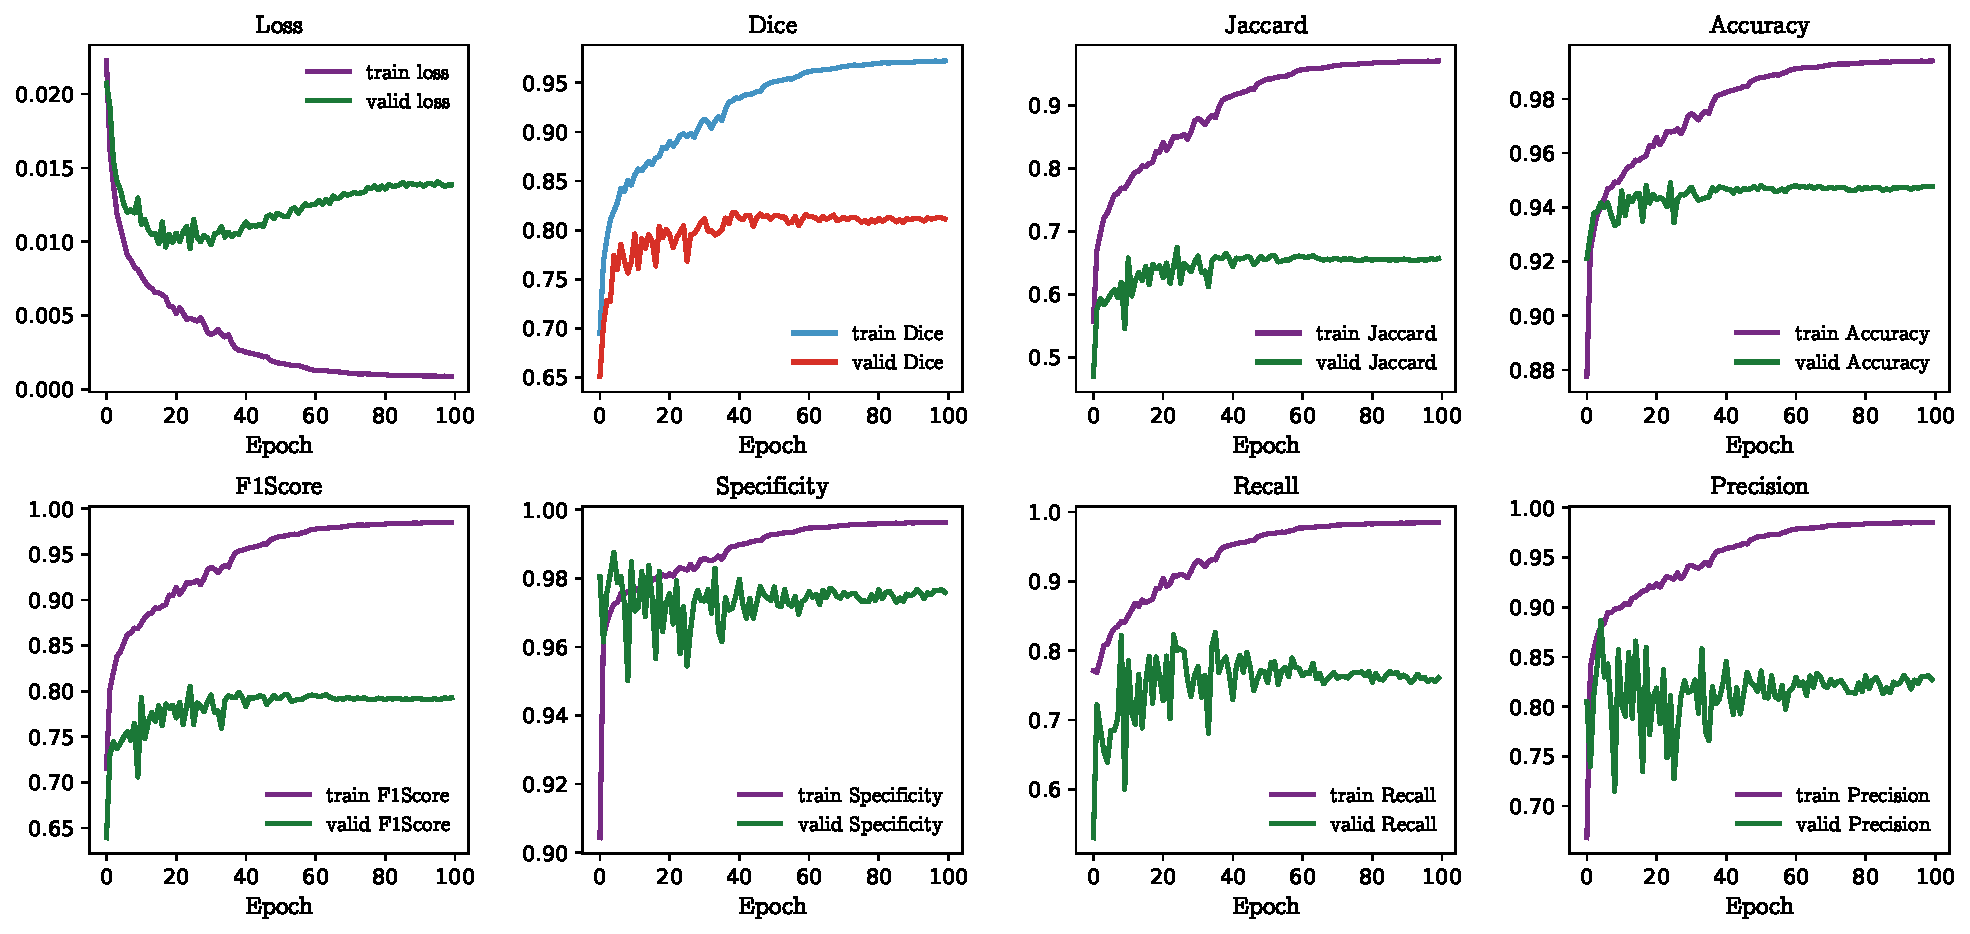
\includegraphics[width=\textwidth]{fig/attunet_metrics.pdf}
    \caption{Attention U-Net在训练过程中的性能指标变化曲线}
    \label{fig:attunet}
\end{figure}

综上,Attention U-Net 作为一种低改动高收益的改进方案,在保持 U-Net 结构主体不变的前提下,即可在 ISIC 2018 数据集上实现 Dice、Recall 等核心指标的全面跃升,且具备更快的收敛速度与更强的训练稳定性。

\subsubsection{AAH U-Net模型的构建与性能验证}

基于前文中消融实验的实验分析和结论,本研究进一步将注意力机制、数据增强策略和混合损失函数这三种有效改进方案进行整合,构建出综合模型AAH U-Net(Attention-Augmentation-HybridLoss U-Net),并与基准模型进行实验对比评估。如表~\ref{tab:model_summary} 所示,AAH U-Net模型在 ISIC 2018 验证集上实现了显著的性能提升。核心指标 Dice 提高了 8.2 个百分点,F1-score 与 IoU 同步提升超过 10\%,而验证损失降低幅度高达 23\%。更重要的是,该方案同时提升了 Recall(+0.133)与 Precision(+0.017),表明模型在降低漏检的同时并未引发误检恶化,这种 Precision–Recall 的双向改善打破了常见的性能权衡瓶颈。

\begin{longtable}{lccccc}
    \caption{各模型在验证集上的主要性能指标横向对比(取最佳 Epoch)}
    \label{tab:model_summary} \\
    \toprule
    指标(Val) & 基准模型 & Augment U-Net & Attention U-Net & HybridLoss U-Net & AAH U-Net \\
    \midrule
    \endfirsthead

    \multicolumn{6}{c}%
    {\tablename\ \thetable\ -- \textit{续表}} \\
    \toprule
    指标(Val) & 基准模型 & Augment U-Net & Attention U-Net & HybridLoss U-Net & AAH U-Net \\
    \midrule
    \endhead

    \bottomrule
    \endfoot

    Dice        & 0.7469 & 0.7624 & 0.818 & 0.752 & \textbf{0.829} \\
    F1-score    & 0.7299 & 0.7481 & 0.814 & 0.740 & \textbf{0.814} \\
    Jaccard     & 0.5747 & 0.5939 & 0.665 & 0.588 & \textbf{0.687} \\
    Precision   & 0.8262 & 0.7429 & 0.808 & 0.776 & \textbf{0.843} \\
    Recall      & 0.6537 & 0.6816 & 0.791 & 0.708 & \textbf{0.787} \\
    Accuracy    & 0.9362 & 0.9399 & 0.948 & 0.934 & \textbf{0.950} \\
    Specificity & \textbf{0.9791} & 0.9772 & 0.9719 & 0.969 & 0.977 \\
    Val-Loss $\downarrow$ & 0.01150 & 0.01011 & 0.0105 & 0.0113 & \textbf{0.00885} \\
\end{longtable}

图~\ref{fig:all_in_is_art}所展示的AAH U-Net模型训练过程也表现出和Attention U-Net模型一样优异的收敛性和稳定性。但相较于Attention U-Net,AAH U-Net的Train–Val Dice差值从 0.089 降至 0.082,反映出该策略还整体提升了模型的泛化能力,并未额外引入过拟合风险。

\begin{figure}[!htbp]
    \centering
    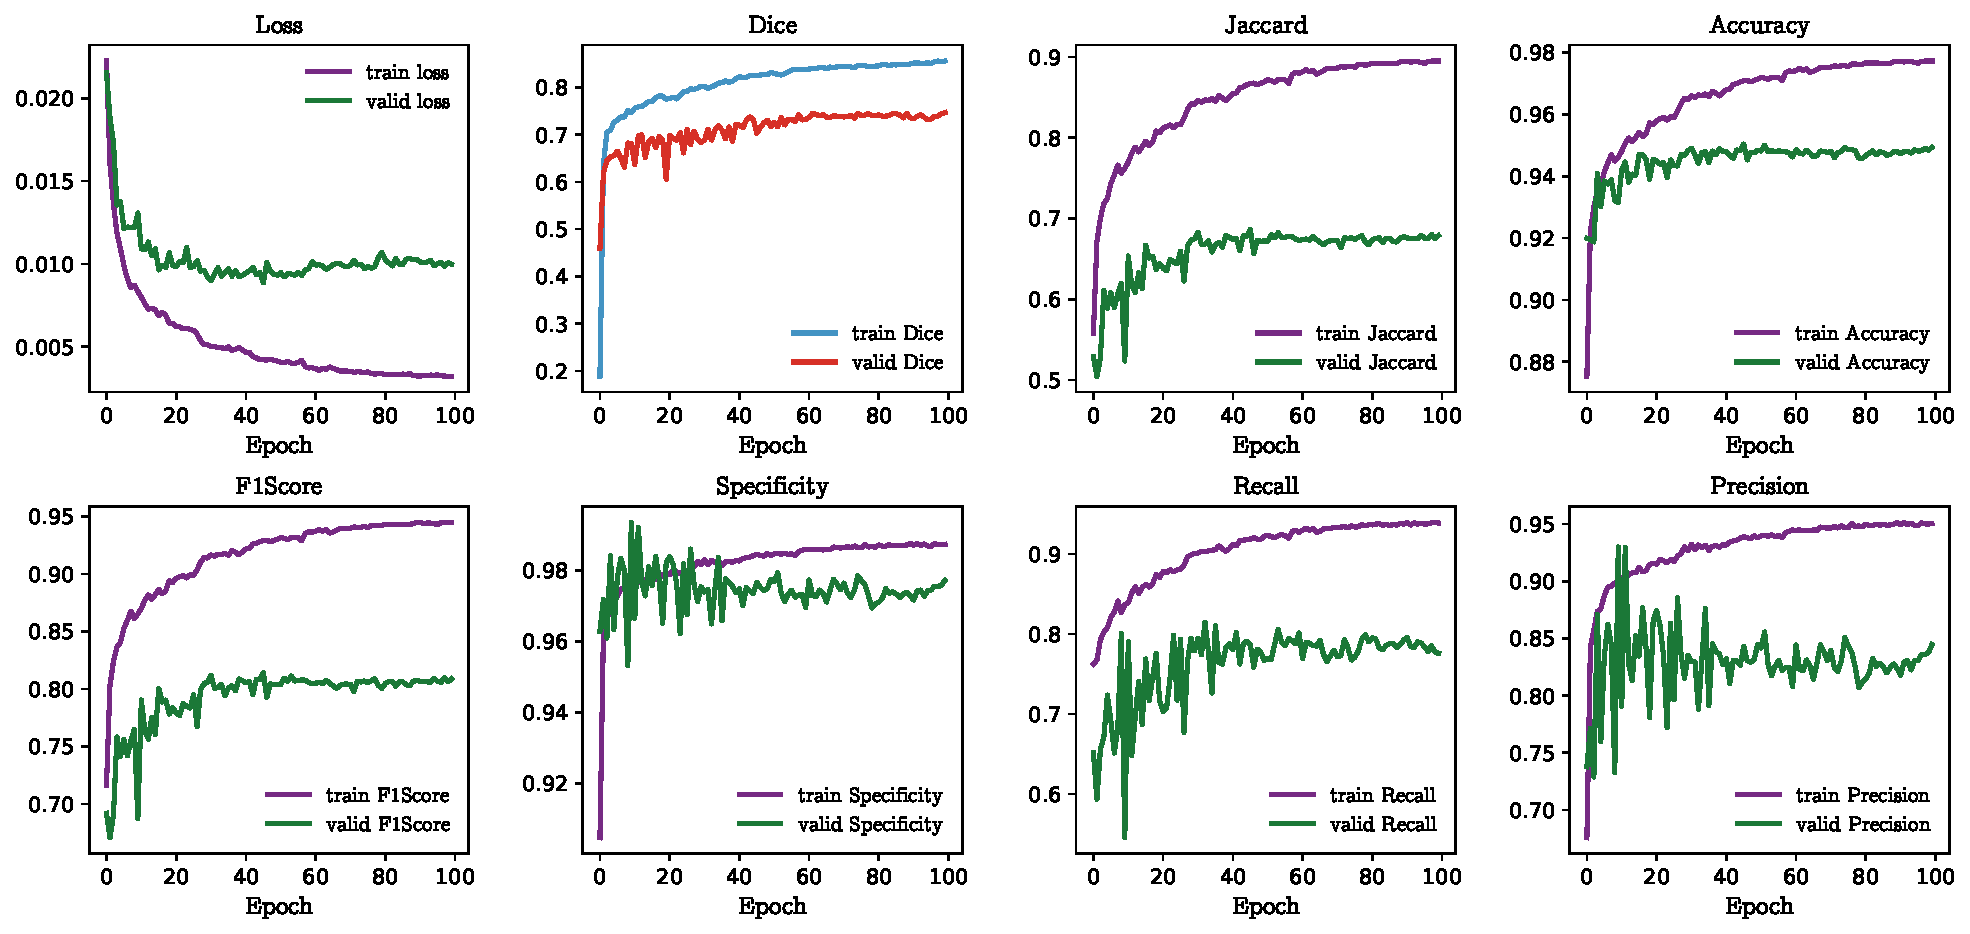
\includegraphics[width=\textwidth]{fig/allin_unet_metrics.pdf}
    \caption{AAH U-Net训练过程中的性能变化曲线}
    \label{fig:all_in_is_art}
\end{figure}

图~\ref{fig:box_img}是消融实验中7个模型在验证集上的Dice系数分布箱式图。从图中我们可以直观看到,与其他模式的箱体相比,AAH U-Net的箱体位置最高(中位线约在0.81),且箱体高度极小(0.79\textasciitilde0.83),表明AAH U-Net模型的分割性能最好,训练过程稳定、收敛快。同时,AAH U-Net的箱体上下须线也最短,只有零散的离群点为初始阶段训练不稳定的结果,表明模型整个训练周期性能非常集中,没有严重震荡。

\begin{figure}[!htbp]
    \centering
    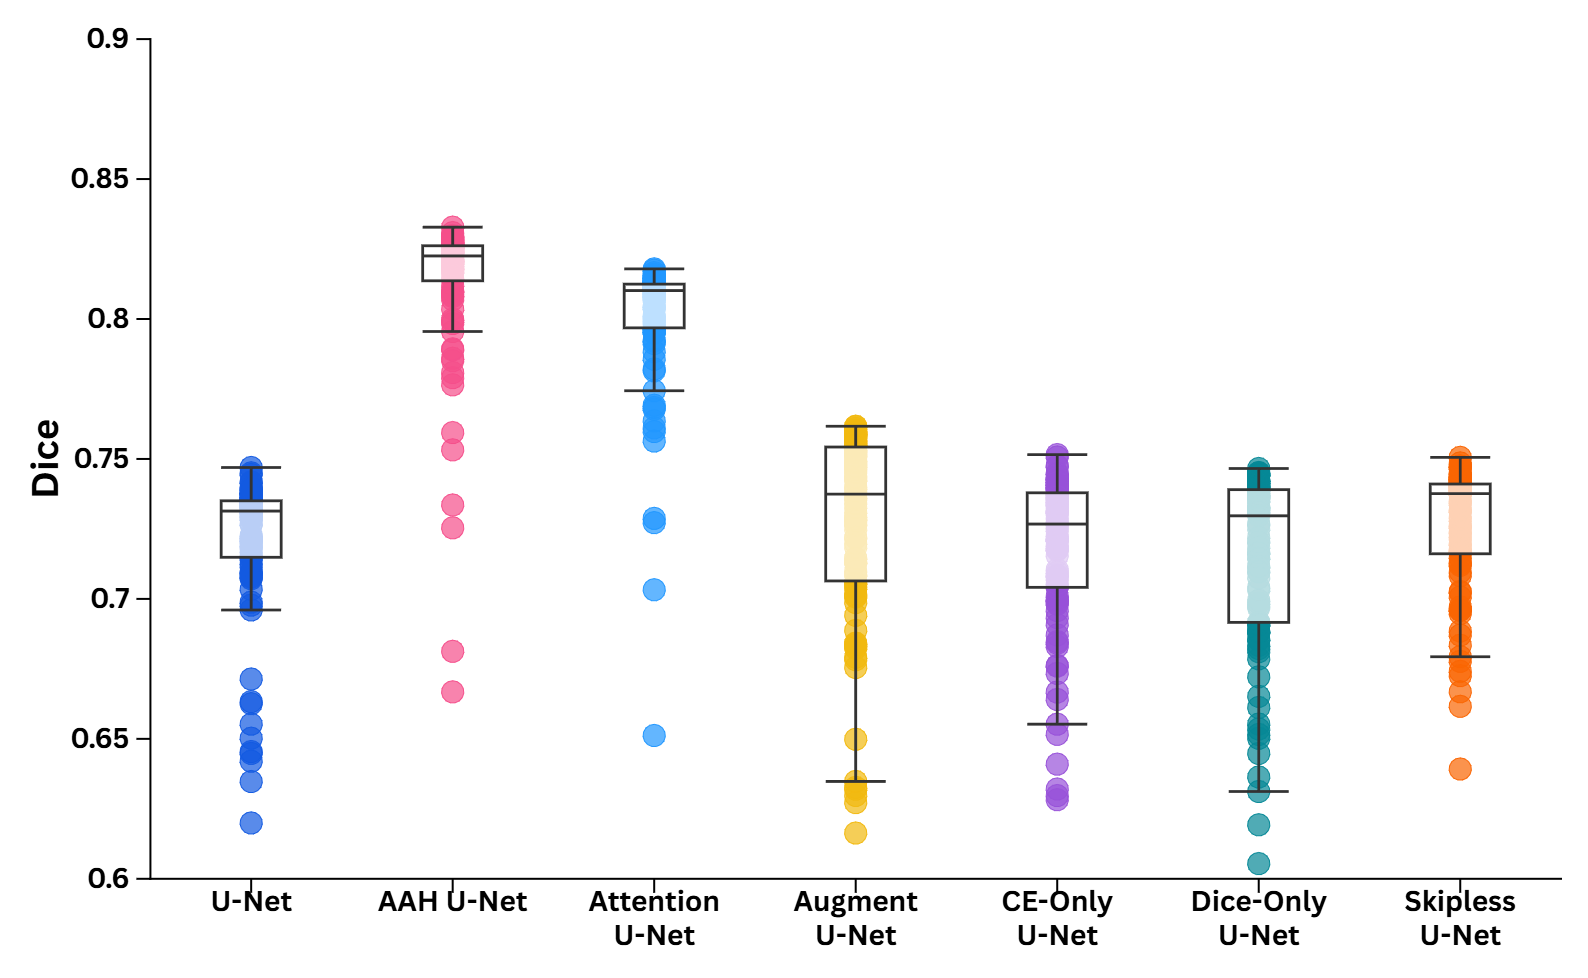
\includegraphics[width=0.8\textwidth]{fig/box_plot@2x.png}
    \caption{各消融模型训练Dice系数分布箱式图}
    \label{fig:box_img}
\end{figure}

反观Augment U-Net和两个采用单一损失函数的U-Net模型,箱体高度明显更高,且下须更低,表明这些模型训练过程中的波动比较大,收敛过程更慢。而通过与Attention U-Net模型的箱体对比发现,Attention U-Net的箱体高度略高于AAH U-Net,箱体位置略低于AAH U-Net,说明采用数据增强策略和混合损失函数提高了模型的鲁棒性和分割性能。

为了进一步展示消融实验和增广实验中不同模型的分割性能,在ISIC 2018的测试集中随机抽取了两张数据展示模型分割结果,如图~\ref{fig:ablation_results}所示,其中绿色轮廓线为原数据的真实分割线,蓝色轮廓线为各模型的预测分割线。

\begin{figure}[!htbp]
    \centering
    \begin{subfigure}{\linewidth}
        \centering
        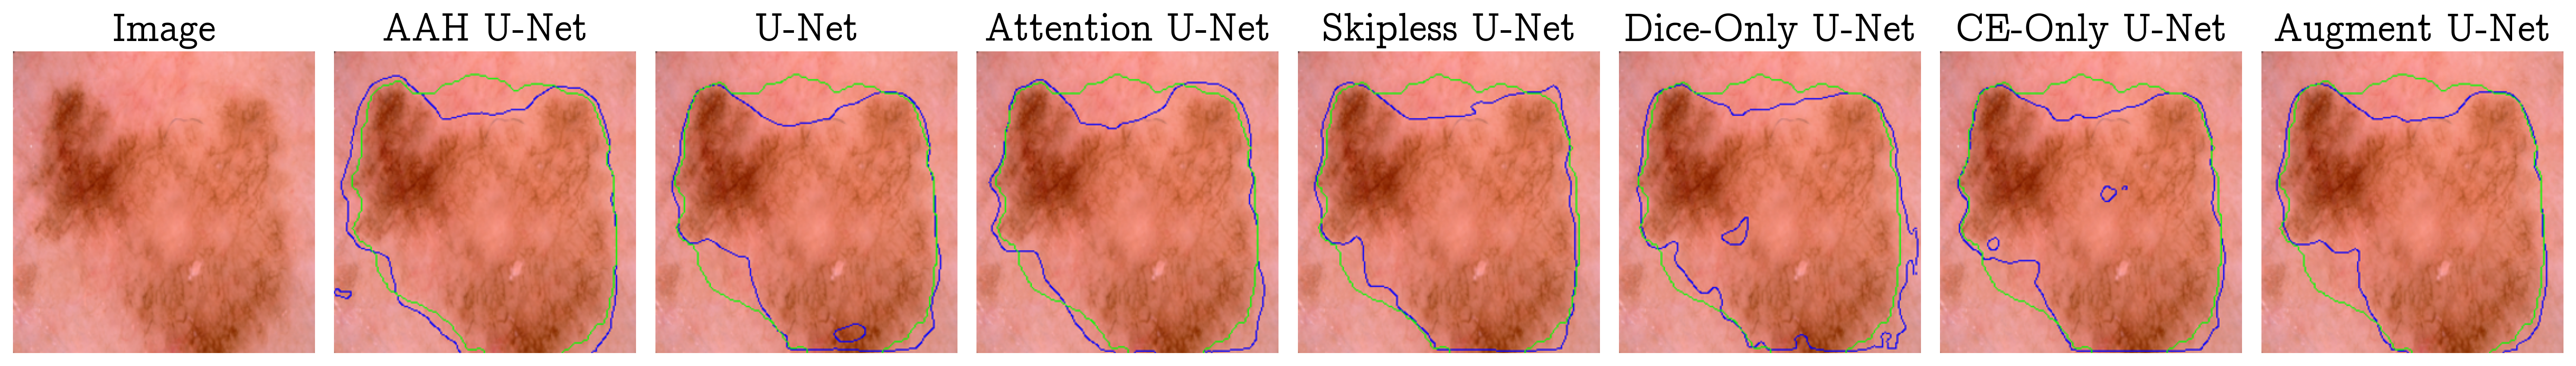
\includegraphics[width=\linewidth]{fig/ablation_compare_row1.png}
    \end{subfigure}
    
    \vspace{0.5em}  % 子图之间留一点间距

    \begin{subfigure}{\linewidth}
        \centering
        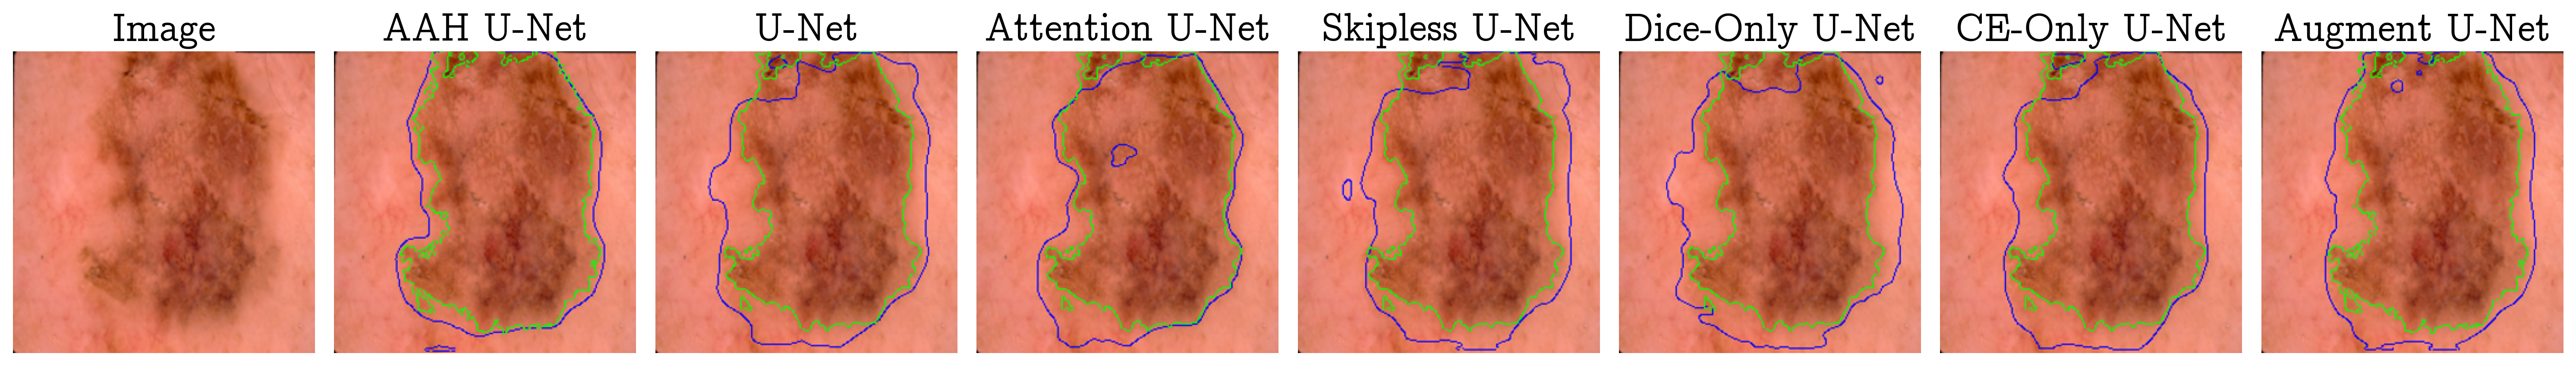
\includegraphics[width=\linewidth]{fig/ablation_compare_row2.png}
    \end{subfigure}

    \caption{消融实验中不同模型在皮肤病变图像上的分割结果对比}
    \label{fig:ablation_results}
\end{figure}

上述性能增益可归因于三项策略间的协同机制。首先,跳跃连接中的注意力机制使解码器端能够动态筛选来自编码器的浅层纹理信息,从而精确重建目标边界并增强定位能力,带动 Recall 与边界 IoU 的显著提升。其次,几何增强操作有效提升了模型对取向和形变的鲁棒性,进一步增强了 Recall 稳定性并降低训练后期指标波动。而引入的混合损失函数则结合了 Dice 对整体重叠度的优化能力与 CE 在像素级别的梯度调控作用,有效控制了假阳性,促使 Precision 不仅恢复而且超过基准水平。三者在机制上的互补性构成了明显的协同效应:数据增强扩大了特征覆盖范围,注意力机制引导网络聚焦于关键信息区域,而混合损失函数则提供了更均衡的 FP/FN 优化路径,最终带来了 Precision–Recall 同时提升的理想结果。

\subsection{泛化性测试}

在第 4.2 节中,我们通过对ISIC 2018皮肤病变数据集的一系列消融实验确定了最佳模型AAH UNet。然而,医学图像分割算法的真正价值并不仅体现在单一数据域的性能,更体现在面对 器官差异、成像模态差异以及标签粒度差异时的跨域鲁棒性。因此,本节将针对LiTS 2017与BraTS 2021这两类与ISIC 2018差异显著的数据集开展泛化性测试。

\subsubsection{LiTS肝脏CT数据集泛化性测试}

针对在LiTS 肝肿瘤 CT 数据集上展开的全量泛化测试,结果显示,在前述ISIC 2018皮肤镜图像分割实验中构建的AAH U-Net模型在 LiTS 验证集中同样展现出卓越的语义分割性能,最终的测试结果如表~\ref{tab:lits_final_metrics}所示。

\begin{table}[!htbp]
    \centering
    \caption{AAH U-Net在 LiTS 验证集上的综合性能指标}
    \label{tab:lits_final_metrics}
    \begin{tabular}{lccccccc}
        \toprule
        指标 & Dice & Jaccard & F1-score & Precision & Recall & Specificity & Accuracy \\
        \midrule
        数值 & 0.893 & 0.757 & 0.862 & 0.822 & 0.905 & 0.9975 & 0.996\\
        \bottomrule
    \end{tabular}
\end{table}

AAH U-Net在LiTS肝肿瘤的分割Dice系数达到了0.893,Jaccard指标为0.757,均优于目前同类二维方法的常规表现,说明该策略在解剖结构更复杂、目标比例更小的医学图像任务中依然具备良好迁移性。

从性能分布来看,模型在多个维度上呈现出一致而稳定的优势。首先,在 Recall 方面取得 0.905 的高分,显示模型在识别小体积病灶时仍具备极强的检出能力,尤其适用于肿瘤早筛与术前评估等高敏感性应用场景。同时 Precision 保持在 0.822 的高位,未出现明显误检恶化,说明模型仍保持合理的类别判别能力。在整体准确率与特异性方面亦分别达到 0.996 与 0.9975,进一步证明模型在背景区域判定方面的稳健性。

图~\ref{fig:LITS_fanhua}展示了全量化模型训练时各指标的变化趋势,不难发现,模型包括Dice系数在内的各个指标的值,在训练和验证阶段几乎持平,显示出极小的过拟合倾向,说明该网络结构在 LiTS 数据集上表现出了非常良好的泛化能力。

\begin{figure}[!h]
    \centering
    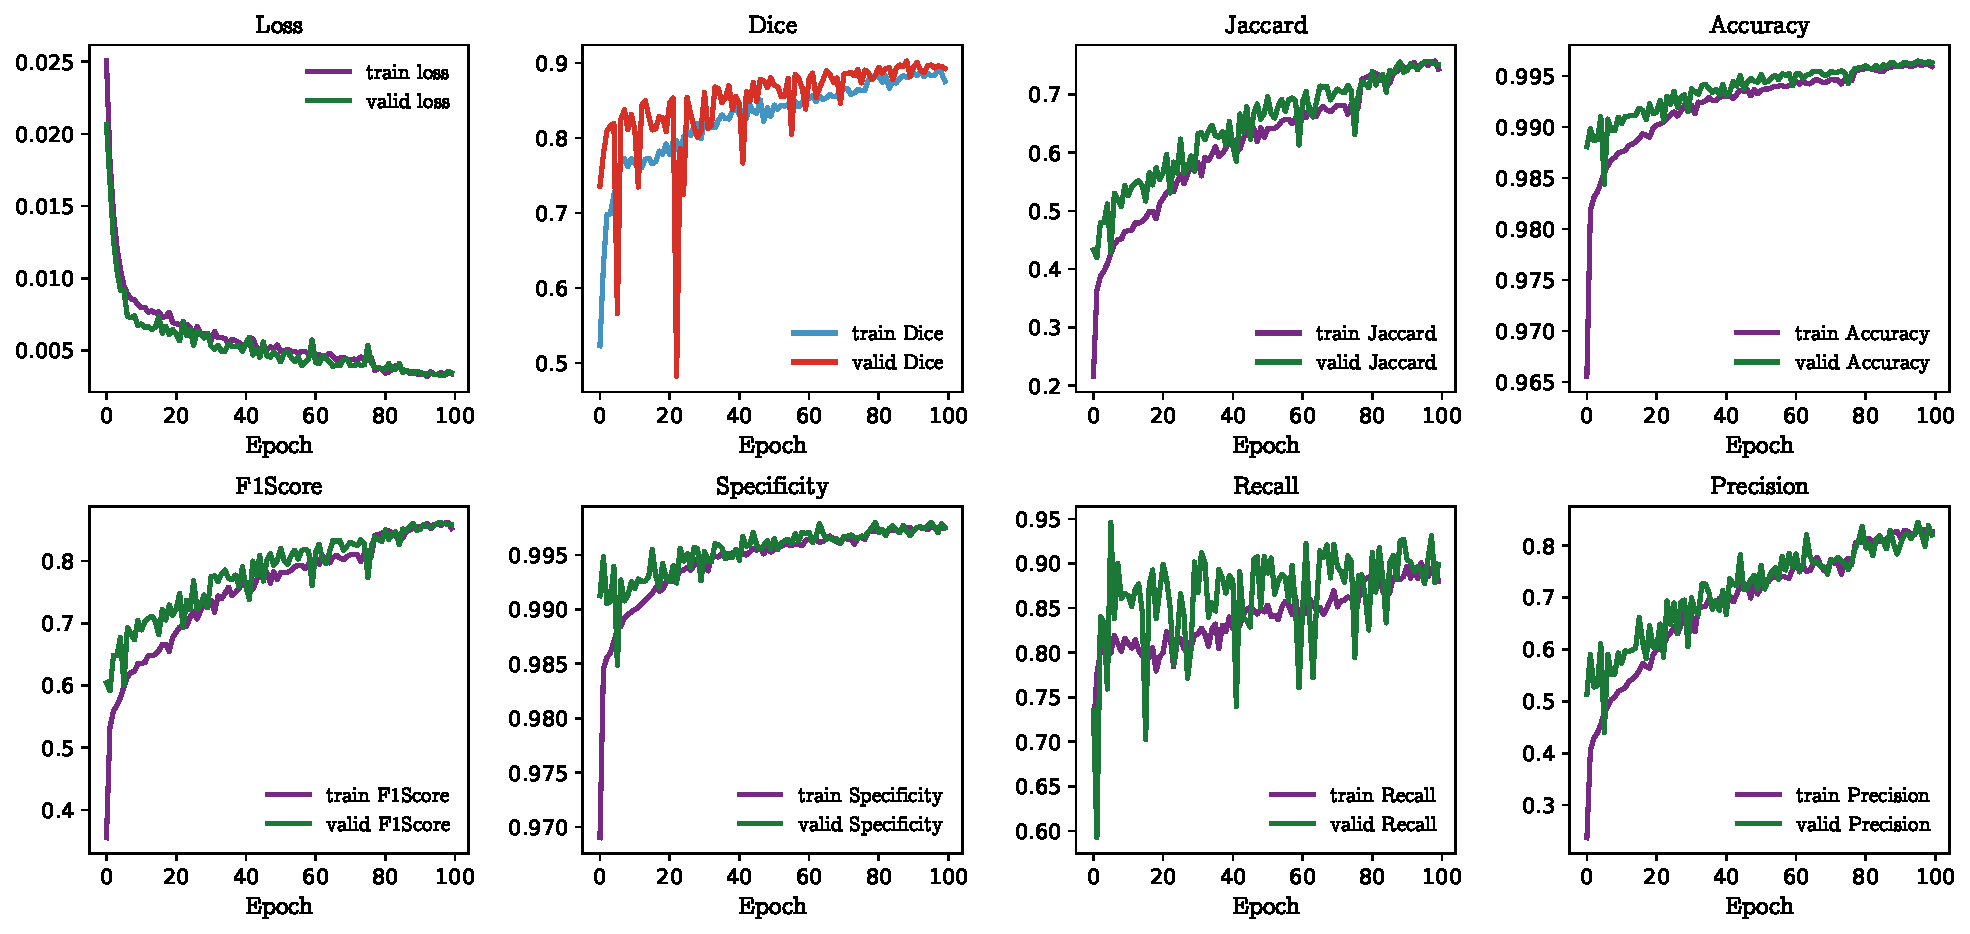
\includegraphics[width=\textwidth]{fig/LITS_fanhua.pdf}
    \caption{AAH U-Net在LiTS数据集上的训练过程}
    \label{fig:LITS_fanhua}
\end{figure}

综上,由注意力机制、数据强化以及混合损失函数构成的U-Net模型不仅在彩色皮肤图像中取得显著性能提升,在结构复杂、前景稀疏的肝脏 CT 场景下亦能稳定泛化,展现了良好的跨域一致性。

\subsubsection{BraTS脑肿瘤MRI数据集泛化性测试}

与前述ISIC 2018数据集和LiTS 2017数据集相比,BraTS 2020数据集作为多模态数据集,每个病例都包含了T1、T1-ce、T2和FLAIR四张MRI序列。同时,如图~\ref{fig:final}所示,对脑肿瘤的语义分割需要同时分割水肿区(ED)、增强肿瘤核心(ET)与坏死区(NCR),形态差异大,类间不平衡显著。

\begin{figure}[!h]
    \centering
    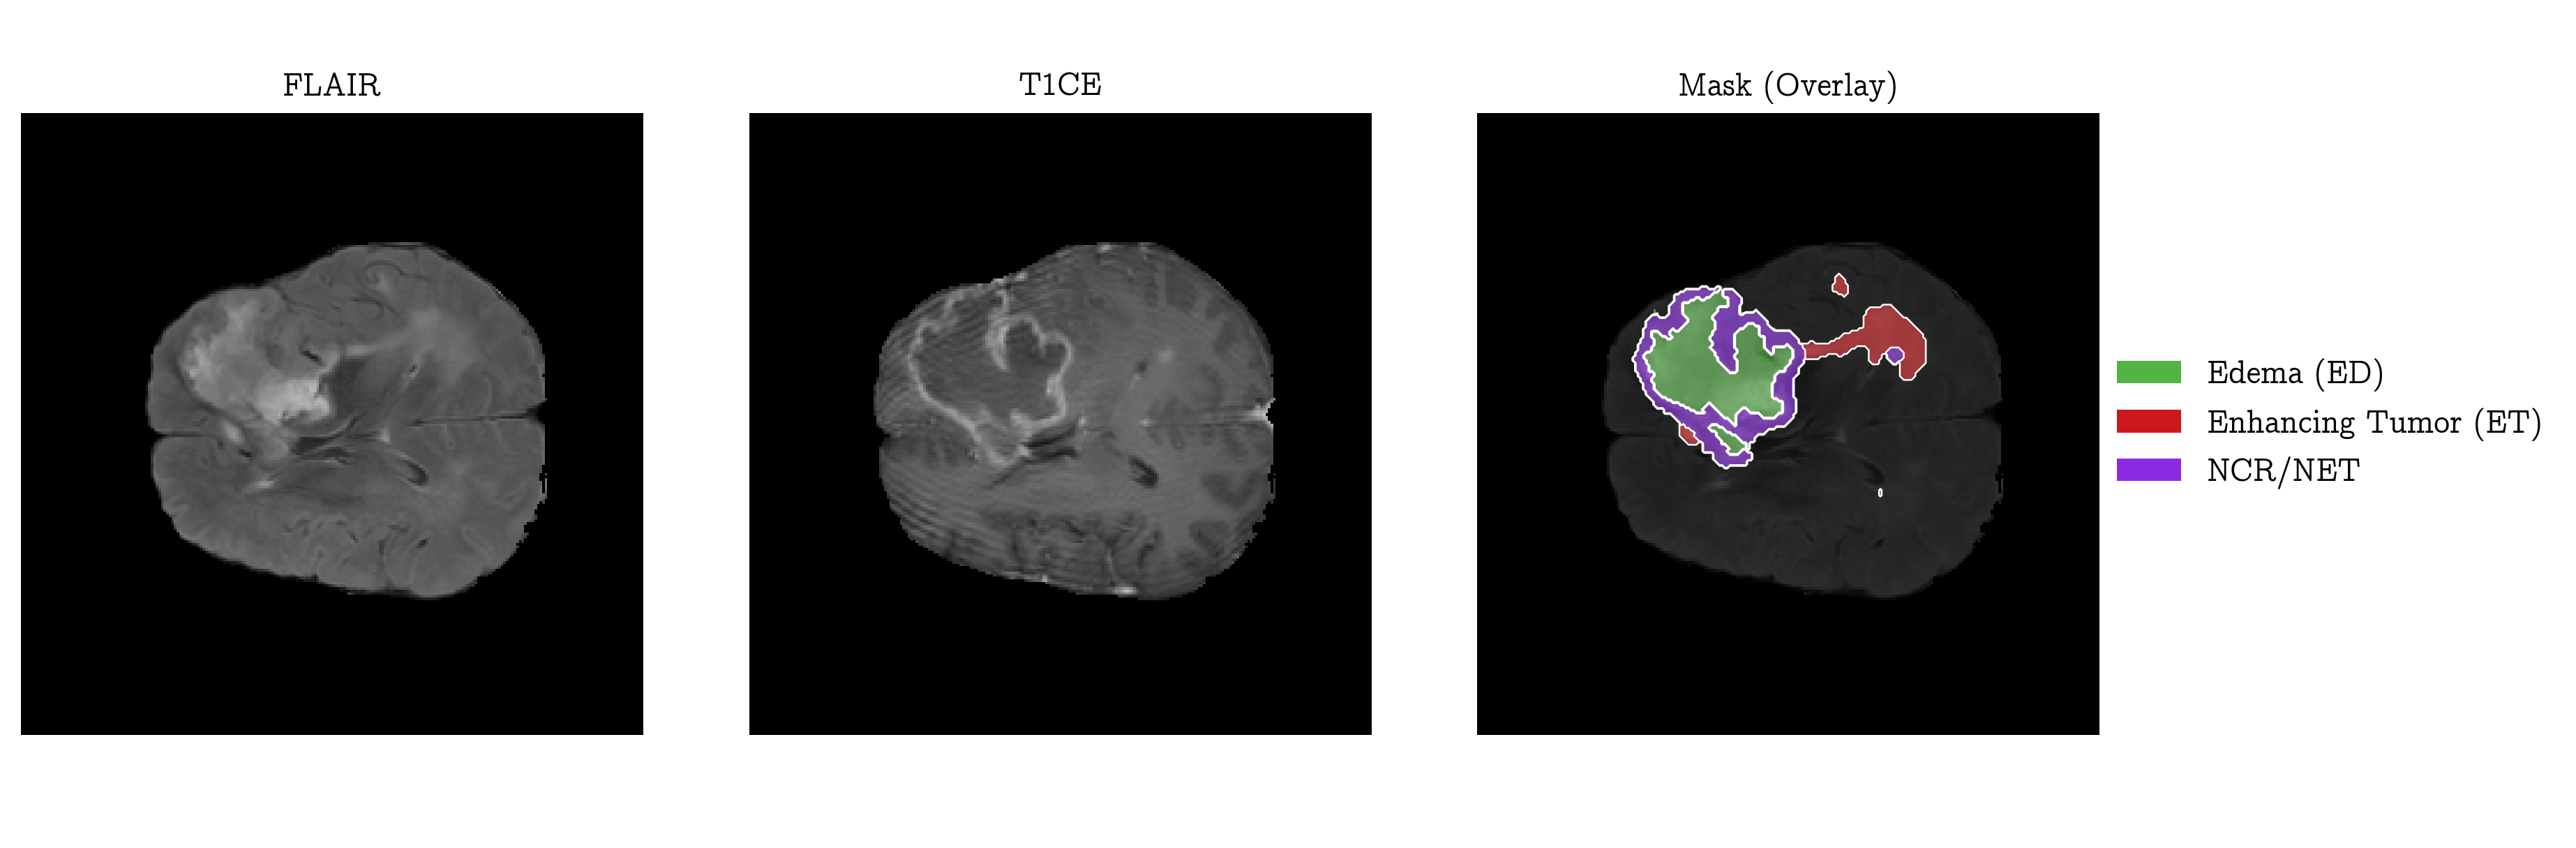
\includegraphics[width=\textwidth]{fig/final_3view_with_right_legend.png}
    \caption{BraTS 脑肿瘤 MRI 示例的多模态输入与语义标签分布}
    \label{fig:final}
\end{figure}

为了得到更广泛的泛化性测试结论,本文选用了BraTS 2020这个高难度数据集进行多模态多分类语义分割任务的泛化性测试。此外,有研究表明对于脑肿瘤语义分割任务,FLAIR和T1-ce这两种模态组合作为输入序列是模型训练最佳的组合选择\cite{buchner2023}。因此,针对BraTS 2020数据集,本研究仅采用FLAIR和T1ce两种模态作为输入序列,同时剔除无标注信息的空白切片以缓解类别极端不平衡问题。最终模型的表现见表~\ref{tab:brain_final_metrics}。

\begin{table}[!h]
    \centering
    \caption{AAH U-Net在 BraTS2020 验证集上的综合性能指标}
    \label{tab:brain_final_metrics}
    \begin{tabular}{lcccccccc}
        \toprule
        指标 & Dice & Dice-ED & Dice-ET & Dice-NCR & Jaccard & F1-score & Precision & Senstivity\\
        \midrule
        数值 & 0.826 & 0.874 & 0.793 & 0.787 & 0.905 & 0.704 & 0.815 & 0.987 \\
        \bottomrule
    \end{tabular}
\end{table}

与 ISIC 2018和 LiTS 2017数据集上指标结果相比,BraTS 2020 的平均Dice系数和三类子区的Dice系数都偏低。这主要是因为模型需要在单幅切片上区分三种形态各异的肿瘤组织,类别之间互斥且界面模糊,难度显著高于前两个二分类任务。同时三类病灶总体体素占脑体积不到 2 \%,前景稀疏导致网络更容易受到类别不平衡和样本噪声的影响。因此,在同等网络与训练策略下,BraTS 2020 的指标略低于 LiTS 2017 与 ISIC 2018 属于预期现象。

尽管如此,模型仍在 BraTS 2020 上的训练曲线稳定收敛。面对多模态 MRI 输入、三类结构区分与极端前景稀疏的情况,本文所采用的注意力增强 U-Net 架构依然在验证集上取得了 0.826 的平均 Dice系数、0.704 的 Jaccard,以及高达 0.987 的 Precision 和 0.986 的 Sensitivity。这些结果表明模型在三类前景之间均具有良好的识别能力,尤其在病灶边界模糊、前景极少的 NCR 区域仍能维持 0.787 的 Dice,展现出较强的小目标分割能力。

不同文献中对 BraTS 2020数据集的语义分割任务的评估略有差异\cite{islam2020,wang2021,menze2015},但已有多个基于标准 2D U-Net 架构的公开实现报告其整体 Dice 通常在 0.62–0.66 区间,本文在不引入深度融合、多分支设计或 3D 卷积的条件下,仅通过轻量注意力门与训练策略优化,即实现了明显的性能突破,体现了方法的良好的跨模态、跨器官和跨类别鲁棒性。

\subsection{方法局限性讨论}

虽然 AAH U-Net在三个数据集的语义分割任务上表现都很优异,但它依旧存在一些问题:

AAH U-Net网络仍采用 2D 切片处理流程,没有充分利用3D体数据的空间上下文的关系。同时,混合损失函数的权重系数固定,在某些情况下,可能并不是最优权重系数,需要通过多次实验比较得到特定任务的最优权重系数。

此外,面对类间极端不平衡、多语义标签的场景,AAH U-Net网络容易先满足大类别的语义分割,导致小类别轮廓可能会被过度平滑甚至完全忽略。这表明AAH U-Net缺乏对极端稀疏类别的专门关注机制及对标签层级结构的建模能力,这也是其在更复杂临床场景中需要优先解决的问题。
